\documentclass[12pt]{beamer}


\usepackage{amsthm, amsmath, amssymb}
\usepackage{tikz}

\usetheme{Frankfurt}
\usecolortheme{default} %beaver
\usecolortheme{default} %orchid 
\usecolortheme{default}

\newcommand{\n}{\newline}
\newcommand{\F}{\ensuremath{\mathbb{F}}}
\newcommand{\Z}{\ensuremath{\mathbb{Z}}}
\renewcommand{\O}{\ensuremath{\mathcal{O}}}

\DeclareMathOperator{\End}{End}

\definecolor{darkgreen}{RGB}{0, 150, 0}

\AtBeginSection[]{
 \frame{\tableofcontents[currentsection]}
}

\title{Elliptic curves in Nemo}

\date{07/01/17}
\author{Jean Kieffer}
\institute{\'Ecole normale sup\'erieure de Paris \& INRIA}

\begin{document}

\frame[plain]{\titlepage}

\frame{\tableofcontents}

\section{Context}

\begin{frame}
 %Couveignes-R-S
 %Such an action arises from elliptic curves
 \frametitle{Key exchange from hard homogeneous spaces}
 Let $G$ be an abelian group acting on a set $X$ with some given point $x_0$. If the action is
 \begin{itemize}
  \pause
  \item easy to compute (polynomial time),
  \pause
  \item hard to invert (exponential time?),
  \pause
 \end{itemize}
 then there is an analogue of the Diffie--Hellman key exchange \cite{Couv}.
 
 \vspace{-5mm}
 \begin{center}
  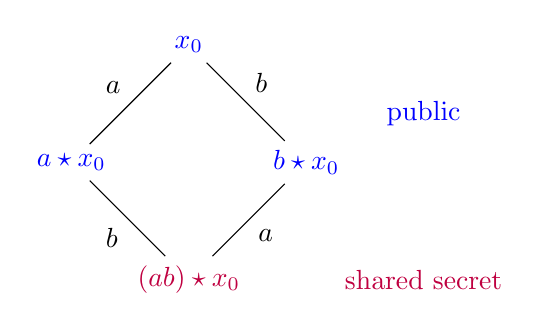
\begin{tikzpicture}[node distance=6em]
   \node(ab) [color=purple] {$(ab) \star x_0$};
   \node(a) [above left of=ab, color=blue] {$a\star x_0$};
   \node(b) [above right of=ab, color=blue] {$b\star x_0$};
   \node(id) [above left of=b, color=blue] {$x_0$};
   \node(p) [below right of=b, color=purple] {shared secret};
   \node(P) [above of=p, color=blue] {public};
   \draw[]
    (ab) edge[auto] node{$b$} (a)
    (b) edge[auto] node{$a$} (ab)
    (a) edge[auto] node{$a$} (id)
    (id) edge[auto] node{$b$} (b);
  \end{tikzpicture}
 \end{center}
\end{frame}

\begin{frame}
 \frametitle{The Couveignes--Rostovtsev--Stolbunov scheme}
 
 \begin{alertblock}{Question}
  Where can we find such an action?
 \end{alertblock}
 
 \pause
 
 \begin{block}{Answer \cite{Couv}, \cite{RoSt}}
  Use the action of a class group on a set of isogenous elliptic curves.
 \end{block}
 
 \pause
 
 \begin{block}{Goals}
   \begin{itemize}
    \item Explain what this means
    \item Describe the computations needed
    \item Discuss our EllipticCurves module for Nemo.
   \end{itemize}
 \end{block}
\end{frame}

\section{An example in isogeny-based cryptography}

%Insert outline

\subsection{Basics}

\begin{frame}
 %Elliptic curves and isogenies
 \frametitle{Elliptic curves over $k$}
 \begin{itemize}
  \item \emph{Elliptic curves} over a field $k$ are algebraic curves that have an abelian group structure, e.g.
  $$\begin{aligned}
  E_1\ &:\ y^2 + a_1 xy  = x^3 + a_2x^2 + a_4x + a_6 \\
  E_2\ &:\ y^2  = x^3 + ax + b \\
  E_3\ &:\ B y^2  = x^3 + Ax^2 + x. 
  \end{aligned}$$
  
  Weierstrass, Short Weierstrass and Montgomery forms, respectively.  
  
  \pause
  
  \item \emph{Isogenies} are nonzero morphisms. Our isogenies will be defined over $k$. As rational maps, they have \emph{degrees}.
 \end{itemize}

 
\end{frame}


\begin{frame}
 %Isogenies as subgroups
 \frametitle{Isogenies are subgroups}
 
 \alert{
  From now on, $k = \F_p$ is a prime finite field.
 }
  
 \pause 
 
 
 Let $E/k$ be an elliptic curve, and $\ell\neq p$ be an odd prime. Giving the following is equivalent :
 \begin{itemize}
  \pause
  
  \item An isogeny $E\to E'$ of degree $\ell$
  
  \pause
  
  \item Its kernel, which is a cyclic subgroup of $E$ of order $\ell$
  
  \pause
  
  \item A polynomial of degree $\frac{\ell - 1}{2}$ in $x$ defining the kernel.
 \end{itemize}
 
 \pause
 \vspace{5mm}
 
 If we know this \emph{kernel polynomial}, we can easily find $E'$ using \alert{V\'elu's formulas}.

\end{frame}


\begin{frame}
 
 \frametitle{Action of the class group}
 
 \vspace{-3mm} 
 \begin{block}{Proposition}
  Let $E/\F_p$ be an ordinary elliptic curve.
  \begin{itemize}
   \item The ring $\End(E)$ is isomorphic to a quadratic order $\O$.
   \item For each prime number $\ell$, there are either 2 (split case), 1 (ramified case) or 0 (inert case) ideals in $\O$ of norm $\ell$. \newline
    \alert{From now on, $\ell$ will always be prime, odd and split.}
   \item Ideal of norm $\ell$ = tuple $(\ell, v)$, $v\in \Z/\ell\Z$.
   \item There is an action on the set of elliptic curves with CM by $\O$. Ideals of norm $\ell$ act as $\ell$-isogenies.
   \item This action is simply transitive.
  \end{itemize}
 \end{block}
 
 \pause
 \vspace{-1mm}
 \begin{alertblock}{Question}
  How can we compute this action ?
 \end{alertblock}

\end{frame}




\subsection{Computations}

\begin{frame}
 \frametitle{Main algorithm}
 
 \vspace{-3mm}
 \begin{alertblock}{Problem}
  Given $E/\F_p$ and a prime $\ell\neq p$, how can we compute the curves linked to $E$ by an $\ell$-isogeny?
 \end{alertblock}

 \pause
 \vspace{-1mm}
 \begin{block}{Most general idea}
  Let $\Phi_\ell(X, Y)$ be the $\ell^{th}$ classical modular polynomial. The two roots $j_1, j_2$ of
  $$\Phi_\ell(j(E), Y)$$
  are the $j$-invariants of the neighbors of $E$. To choose the one corresponding to an ideal $(\ell, v)$:
  \begin{itemize}
   \item compute the kernel $K(x)$ of the isogeny $E\to j_1$
   \item check if the Frobenius acts on it as scalar mult. by $v$:
    \vspace{-4mm}
    $$(x^p, y^p) \overset{?}{=} [v]\cdot (x, y) \mod K(x) \text{ and curve equation}.$$
  \end{itemize}
 \end{block}
\end{frame}

\begin{frame}
 \frametitle{Bostan--Morain--Salvy--Schost \cite{BMSS}}
 
 \vspace{-3mm}
 \begin{alertblock}{Question}
  How can we compute the kernel $K(x)$ of $\phi\ :\ E \to j_1$ ?
 \end{alertblock}
 
 \pause
 
 \begin{block}{Idea}
  If $\phi$ is \emph{normalized}, the rational fraction defining it satisfies a simple differential equation.
 \end{block}
 
 \pause
 
 \begin{block}{Algorithm}
  \begin{itemize}
   \item Normalize $\phi$ (involves evaluating modular polynomials)
   \item Solve this ODE in power series up to a certain precision with a \alert{Newton iteration}
   \item Recover $K(x)$ using the Berlekamp--Massey rational reconstruction algorithm.
  \end{itemize}
 \end{block}
\end{frame}



\begin{frame}
 \frametitle{Another solution}
 
 \vspace{-3mm}
 
 \begin{alertblock}{Problem}
  Given $E/\F_p$ and a prime $\ell\neq p$, how can we compute the curves linked to $E$ by an $\ell$-isogeny?
 \end{alertblock}

 Finding roots of modular polynomials is costly : $\Phi_\ell(X, Y)$ has degree $\ell + 1$ in both variables. 
 
 \pause
 
 \begin{block}{More specific idea}
  Suppose that for some $d$, $K$ is the only subgroup of order $\ell$ in $E$ whose points are defined over $\F_{p^d}$. 
  \begin{itemize}
   \item Look for $\ell$-torsion points over this field to find $K$, using scalar multiplications
   \item Compute the curve $E/K$ using V\'elu's formulas.
  \end{itemize}
  The isogeny $E\to E/K$ has degree $\ell$.
 \end{block}
\end{frame}


\begin{frame}
 \frametitle{Finding adequate curves}
 
 This second method is only efficient with small-degree extensions.
 
 Not every curve satisfies the conditions before for small $d$: we have to look for adequate curves.
 
 In practice, we have to use both algorithms, general and specific.

\end{frame}

\section{The EllipticCurves module for Nemo}


\subsection{Contents}

\begin{frame}
 \frametitle{What we would like Nemo to do}
 
 In the general method:
  \begin{itemize}
   \item Define elliptic curves over finite fields and general rings
   \item Define isogenies, sacalar multiplication and isomorphisms
   \item Find roots of polynomials over finite fields
   \item Solve ODEs in power series with Newton iterations
   \item Berlekamp--Massey
  \end{itemize}
   
  \pause
  
  In the specific method:
  \begin{itemize}
   \item Define points on elliptic curves
   \item Arithmetic operations on elliptic curves
   \item Extensions of finite fields.
  \end{itemize}

\end{frame}



\begin{frame}
 %Elliptic curves and isogenies in Nemo : abstract types, etc.
 \frametitle{Types for curves}
 
 We want both Weierstrass models (all curves have one) and Montgomery models (efficient arithmetic).
 
 \pause
 \vspace{-6mm}
 \begin{center}
  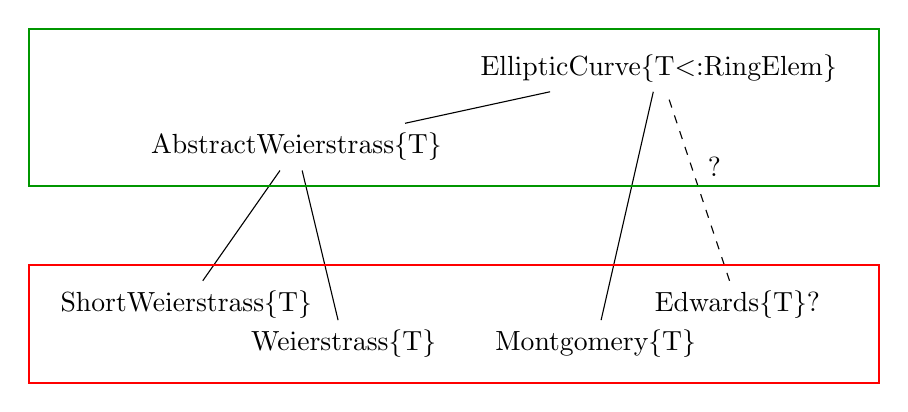
\begin{tikzpicture}[xscale=2, yscale=1]
   \draw[]
    (0,0) node(1) {EllipticCurve\{T$<:$RingElem\}}
    (-2.3,-1) node(2) {AbstractWeierstrass\{T\}}
    (-3,-3) node(3) {ShortWeierstrass\{T\}}
    (-2, -3.5) node(4) {Weierstrass\{T\}}
    (-0.4, -3.5) node(5) {Montgomery\{T\}}
    (0.5, -3) node(6) {Edwards\{T\}?};
   
   \draw[]
    (1) edge (2)
    (3) edge (2)
    (4) edge (2)
    (5) edge (1);
   
   \draw (6) edge[dashed]  node[above right] {?} (1);
   
   %Abstract and concrete
   
   \draw[thick,darkgreen] (-4, -1.5) rectangle (1.4, 0.5);
   \draw[thick,red] (-4, -4) rectangle (1.4, -2.5);
 
  \end{tikzpicture}
 \end{center}
 \vspace{-3mm}
 E.g. {\tt j-invariant} is defined for the EllipticCurve type, while
 {\tt a-invariants} is only defined for AbstractWeierstrass.
\end{frame}

\begin{frame}
 %Types for maps
 \frametitle{Types for maps}
 
 Maps can be isomorphisms between different models (evaluate on points), isogenies (compute image and kernels), scalar multiplications (both?).
 
 \pause
 \begin{center}
  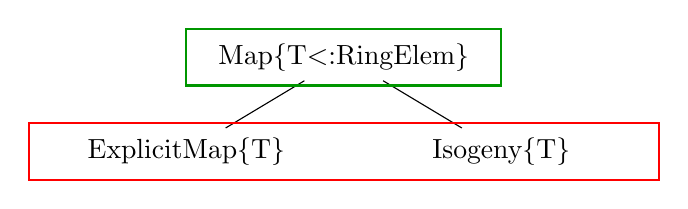
\begin{tikzpicture}[x=2cm, y=1.2cm]
 
  \draw[]
   (0,0) node(1) {Map\{T$<:$RingElem\}}
   (-1,-1) node(2) {ExplicitMap\{T\}}
   (1, -1) node(3) {Isogeny\{T\}};
  
  \draw[]
   (1) edge (2)
   (1) edge (3);
  
  %Abstract and concrete
  \draw[thick, darkgreen] (-1, -0.3) rectangle (1, 0.3);
  \draw[thick, red] (-2, -1.3) rectangle (2, -0.7);
  \end{tikzpicture}
 \end{center}
 
 \begin{columns}
  \column{0.05\textwidth}
  \column{0.5\textwidth}
   \scriptsize\tt immutable ExplicitMap\{T\} <: Map\{T\}\newline
	\ \quad domain::EllipticCurve\{T\} \newline
	\ \quad image::EllipticCurve\{T\} \newline
	\ \quad map::Function\newline
	end  \newline
  \column{0.5\textwidth}
  \scriptsize\tt
  immutable Isogeny\{T\} <: Map\{T\}\newline
	\ \quad domain::EllipticCurve\{T\}\newline
	\ \quad degree::Integer\newline
	\ \quad kernel::PolyElem\{T\}\newline
	\ \quad image::EllipticCurve\{T\}\newline
	end
 \end{columns}
\end{frame}

\begin{frame}
 %Types for points
 \frametitle{Types for points}
 \begin{itemize}
  \item  Should points be attached with a curve?
  \item Arithmetic on Montgomery curves is much more efficient using only $x$-coordinates.
 \end{itemize}
 
 \pause
 \begin{center}
  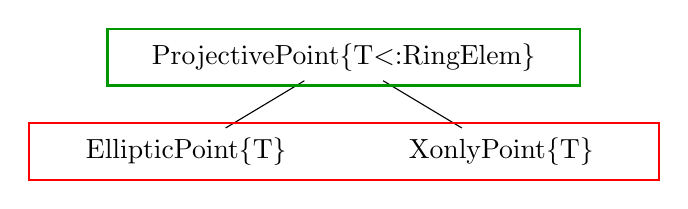
\begin{tikzpicture}[x=2cm, y=1.2cm]
 
  \draw[]
   (0,0) node(1) {ProjectivePoint\{T$<:$RingElem\}}
   (-1,-1) node(2) {EllipticPoint\{T\}}
   (1, -1) node(3) {XonlyPoint\{T\}};
  
  \draw[]
   (1) edge (2)
   (1) edge (3);
  
  %Abstract and concrete
  \draw[thick, darkgreen] (-1.5, -0.3) rectangle (1.5, 0.3);
  \draw[thick, red] (-2, -1.3) rectangle (2, -0.7);
  \end{tikzpicture}
 \end{center}
 
 \begin{columns}
  \column{0.2\textwidth}
  \column{0.5\textwidth}
   \scriptsize\tt type EllipticPoint\{T\} <: ProjectivePoint\{T\}\newline
	X::T\newline
	Y::T\newline
	Z::T\newline
	curve::EllipticCurve\{T\} \newline
end
  \column{0.5\textwidth}
  \scriptsize\tt type XonlyPoint\{T\} <: ProjectivePoint\{T\}\newline
    X::T \newline
    Z::T \newline
    curve::MontgomeryCurve\{T\} \newline
end \newline
 \end{columns}
\end{frame}


\begin{frame}
 %Contents
 \frametitle{What EllipticCurves can do}
 
 \begin{itemize}
  \item Define curves, points and maps, check for equality and validity
  \item Basic functions such as invariants
  \item Compute isomorphisms between different models
  \item Generic arithmetic on Weierstrass/Montgomery curves
  \item Efficient $x$-only arithmetic on Montgomery curves
  \item Division polynomials for ShortWeierstrass
  \item Isogeny computations : V\'elu's formulas and the BMSS algorithm for short Weierstrass and Montgomery curves
  \item Modular polynomials (for small $\ell$'s)
  \item Over finite fields : random points, torsion points, computation of Frobenius eigenvalues.
 \end{itemize}
\end{frame}

\subsection{Further development}

\begin{frame}
 %Useful things
 \frametitle{Useful things that should be done elsewhere}
 In finite fields :
 \begin{itemize}
  \item Multiplicative orders
  \item Random elements
  \item Square roots
  \item Roots of polynomials and irreducible polynomials
  \item Field extensions over \emph{prime} fields
 \end{itemize}
 Others:
 \begin{itemize}
  \item Derivatives of multivariate polynomials
 \end{itemize}
\end{frame}


\begin{frame}
 \frametitle{Further possible development}
 \begin{itemize}
  \item Call (system) PARI to compute the cardinality of curves over finite fields
  \item Compute modular polynomials/equations on the fly?
  \item Zeta functions?   
  \item Have $p$-adic numbers to compute isogenies in small characteristic?
  \item Go down the arithmetic route for elliptic curves over number fields or local fields?
 \end{itemize}
\end{frame}

\subsection{Some benchmarks}


\begin{frame}
%Three solutions : Nemo, Nemo bis, PARI
\frametitle{Three ways to compute roots over $\F_p$}

At present, there is no direct way to do this in Nemo.

\begin{columns}[t]
 \column{0.33\textwidth}
 \begin{block}{Sol. 1 (Nemo)}
  \scriptsize\tt function roots(P)\n
    A = parent(P) \n
    X = gen(A) \n
    R = ResidueRing(A, P) \n
    Frob = R(X)$\hat{~}$BigInt(p) \n 
    Frob = data(Frob) \n
    g = gcd(Frob - X, P) \n
    fact = factor(g) \n
    ...\quad\# recover roots \n
    end
 \end{block}

 \column{0.33\textwidth}
 \begin{block}{Sol. 2 (Sage/PARI)}
  \scriptsize\tt
  def roots(P):\n
   Q = pari(P) \n
   rts = Q.polrootsmod(p) \n
   return rts.sage()
 \end{block}


 \column{0.33\textwidth}
 \begin{block}{Sol. 3 (Sage)}
  \scriptsize\tt
  def roots(P):\n
    A = P.parent()\n
    X = A.gen()\n
    R = A.quotient(P)\n
    Frob = R(X)**p\n
    Frob = Frob.lift()\n
    g = gcd(Frob, P)\n
    return g.roots()
 \end{block}
\end{columns}

\end{frame}



\begin{frame}[plain]
 %Graph
 \frametitle{Timing results}
 
 %\vspace{-1cm}
 \begin{center}
  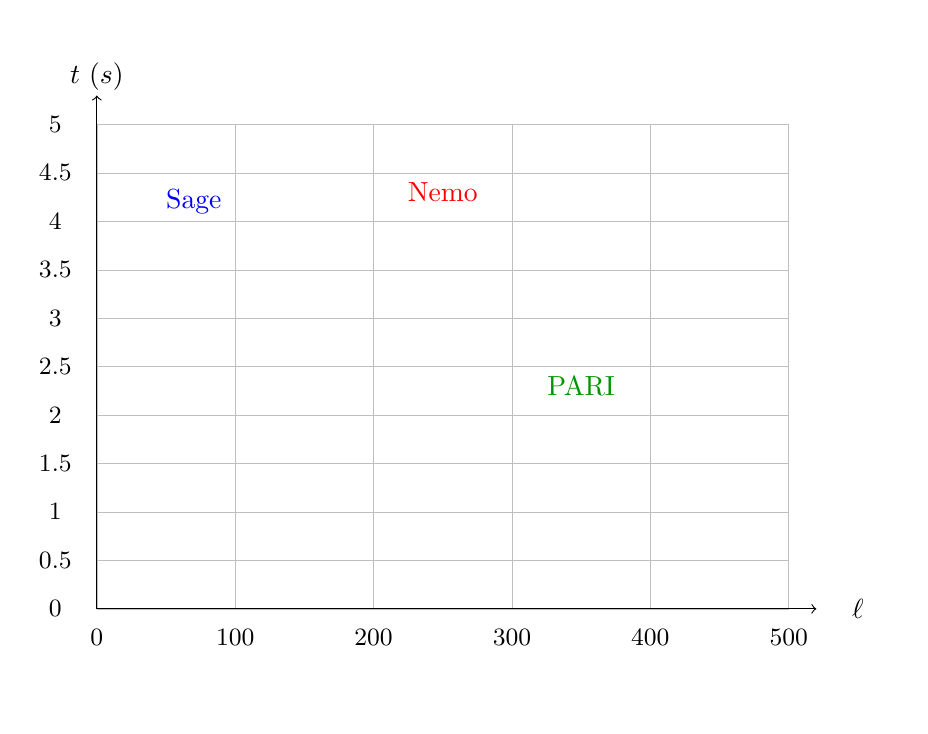
\begin{tikzpicture}[x=0.5, y=35]
   
   \clip (-50,-1) rectangle (580, 6);
   %Curves
   \draw[thick, blue] plot file {sagemod.txt};
   \draw[thick, darkgreen] plot file {parimod.txt};
   \draw[thick, red] plot file {nemomod.txt};
   
   %Grid
   \draw[color=gray!50, very thin] (0,0) grid[xstep = 100, ystep = 0.5] (500, 5);
   \foreach \k in {0,100,...,500}
    \draw  (\k, -0.3) node  {\small\k};
   \foreach \t in {0,0.5,...,5}
    \draw (-30, \t) node {\small \t};
   
   %Axes
   \draw[->] (0,0) -- (0, 5.3);
   \draw[->] (0,0) -- (520, 0);
   \draw (550, 0) node {$\ell$};
   \draw (0, 5.5) node {$t\ (s)$};
   
   %Legend
   \draw[blue] (70, 4.2) node {Sage};
   \draw[darkgreen] (350, 2.3) node {PARI};
   \draw[red] (250, 4.3) node {Nemo};
  \end{tikzpicture}
 \end{center}
\end{frame}





\begin{frame}
%Three solutions : Nemo, Nemo bis, PARI
\frametitle{Three ways to compute scalar multiplications}

\begin{columns}[t]
 \column{0.5\textwidth}
 \begin{block}{Sol. 1 (Nemo)}
  \scriptsize\tt
  E = Weierstrass(...)\n
  Fext, \_ = FiniteField(p$\hat{~}$d, alpha)\n
  Eext = base\_extend(E, Fext)\n
  P = random(Eext)\n
  times(p$\hat{~}$d, P)
 \end{block}

 %\column{0.33\textwidth}
 \begin{block}{Sol. 2 (Nemo)}
  \scriptsize\tt
  E = Montgomery(...)\n
  Fext, \_ = FiniteField(p, d, alpha)\n
  Eext = base\_extend(E, Fext)\n
  P = randomXonly(Eext)\n
  times(p$\hat{~}$d, P)
 \end{block}


 \column{0.5\textwidth}
 \begin{block}{Sol. 3 (Sage)}
  \scriptsize\tt
  E = EllipticCurve(...)\n
  Fext = FiniteField(p**d, "alpha")\n
  Eext = E.base\_extend(Fext)\n
  P = Eext.random\_element()\n
  C = p**d\n
  C * P
 \end{block}
\end{columns}

\end{frame}


\begin{frame}
 %Graph
 \frametitle{Timing results}
 \vspace{-1cm}
 \begin{center}
  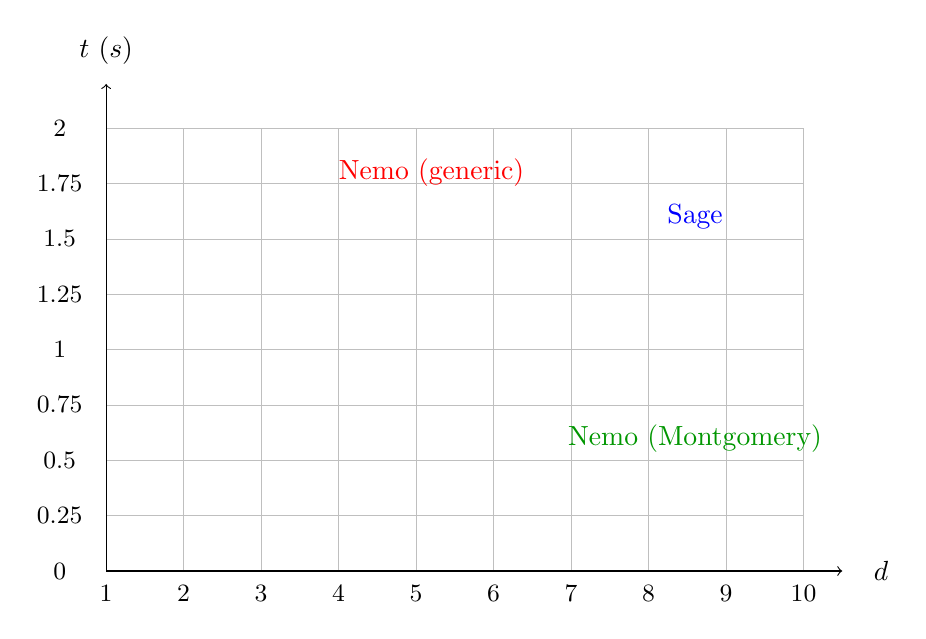
\begin{tikzpicture}[x=28, y=80]
   %Curves
   \draw[thick, blue] plot file {sagetors.txt};
   \draw[thick, red] plot file {generic.txt};
   \draw[thick, darkgreen] plot file {montgomery.txt};
   
   %Grid
   \draw[color=gray!50, very thin] (1,0) grid[xstep = 1, ystep = 0.25] (10, 2);
   \foreach \k in {1,2,...,10}
    \draw  (\k, -0.1) node  {\small\k};
   \foreach \t in {0,0.25,...,2}
    \draw (0.4, \t) node {\small \t};
 
   %Axes
   \draw[->] (1,0) -- (1, 2.2);
   \draw[->] (1,0) -- (10.5, 0);
   \draw (11, 0) node {$d$};
   \draw (1, 2.35) node {$t\ (s)$};
   
   %Legend
   \draw[blue] (8.6, 1.6) node {Sage};
   \draw[darkgreen] (8.6, 0.6) node {Nemo (Montgomery)};
   \draw[red] (5.2, 1.8) node {Nemo (generic)};
  \end{tikzpicture}
 \end{center}
\end{frame}



\section{Conclusion}

\begin{frame}
 %Remarks
 \frametitle{Questions}
 \begin{itemize}
  \item Can we do better to compute roots of polynomials over finite fields?
  \item Can we do better for non-prime finite fields?
 \end{itemize}
\end{frame}

\begin{frame}
 %End
 \frametitle{Take home messages}
 \begin{itemize}
  \item \ldots
 \end{itemize}
\end{frame}

\begin{frame}
 \begin{center}
  \huge{Thank you!}
 \end{center}
\end{frame}


\begin{frame}
 %References
 \frametitle{References}
 \bibliographystyle{plain}
 \bibliography{bibposter}

\end{frame}

\end{document}

